\renewcommand{\theequation}{\theenumi}
\begin{enumerate}[label=\arabic*.,ref=\thesubsection.\theenumi]
\numberwithin{equation}{enumi}
\item  Equal chords of a circle (or of congruent circles) subtend equal angles at the centre. 
\item  If the angles subtended by two chords of a circle (or of congruent circles) at the centre (corresponding centres) are equal, the chords are equal.
\item  The perpendicular from the centre of a circle to a chord bisects the chord. 
\item  The line drawn through the centre of a circle to bisect a chord is perpendicular to the chord.
\item  There is one and only one circle passing through three non-collinear points. 
\item  Equal chords of a circle (or of congruent circles) are equidistant from the centre (or corresponding centres).
\item Chords equidistant from the centre (or corresponding centres) of a circle (or of congruent circles) are equal.
\item  If two arcs of a circle are congruent, then their corresponding chords are equal and conversely if two chords of a circle are equal, then their corresponding arcs (minor, major) are congruent.
\item Congruent arcs of a circle subtend equal angles at the centre. 
\item  The angle subtended by an arc at the centre is double the angle subtended by it at any point on the remaining part of the circle.
\item Angles in the same segment of a circle are equal. \item  Angle in a semicircle is a right angle. 
\item  If a line segment joining two points subtends equal angles at two other points lying on the same side of the line containing the line segment, the four points lie on a circle. 
\begin{enumerate}
\begin{figure}[!ht]
\centering
\resizebox{\columnwidth}{!}{	\begin{tikzpicture}
[scale=2,>=stealth,point/.style={draw,circle,fill = black,inner sep=0.5pt},]

%Triangle sides
\def\a{5}
\def\b{6}
\def\c{4}
\def\R{3.023715784073818}

%Coordinates of A
%\def\p{0.5}
\def\p{((\a^2+\c^2-\b^2)/(2*\a))}
\def\q{{sqrt(\c^2-\p^2)}}

\def\x{((\a^2+\b^2-\c^2)/(2*\a))}
\def\y{{sqrt(\b^2-\x^2)}}

%Labeling points
%\node (A) at ($({((\a^2+\c^2-\b^2)/(2*\a))},{sqrt(\c^2-\x^2)} )$)[point,label=above right:$A$] {};
\node (A) at ($({((\a^2+\c^2-\b^2)/(2*\a))},{sqrt(\c^2-\p^2)} )$)[point,label=below left:$A$] {};
\node (B) at (0, 0)[point,label=below left:$B$] {};
\node (C) at (\a, 0)[point,label=below right:$C$] {};
\node (D) at ($({((\a^2+\b^2-\c^2)/(2*\a))},{sqrt(\b^2-\x^2)} )$)[point,label=below left:$D$] {};
%\node (E) at ($({(\a)}, {((\a)/((\a^2+\b^2-\c^2)/(2*\a))*(sqrt(\c^2-\p^2))})$)[point,label=below right:$E$] {};
%Circumcentre

\node (O) at (2.5,1.70084013)[point,label=above right:$O$] {};

%Drawing triangle ABC
\draw (A) -- node[left] {$\textrm{c}$} (B) -- node[below] {$\textrm{a}$} (C) -- node[above,yshift=2mm] {$\textrm{b}$} (A);

\draw (D) -- node[left] {$\textrm{e}$} (B);
\draw (D) -- node[left] {$\textrm{d}$} (C);

%\draw[dashed] (E) -- node[left] {$\textrm{}$} (B);
%\draw[dashed] (E) -- node[left] {$\textrm{}$} (C);
%Drawing OA, OB, OC
%\draw (O) -- node[left] {$\textrm{R}$} (A);
%\draw (O) -- node[below] {$\textrm{R}$} (B);
%\draw (O) -- node[below] {$\textrm{R}$} (C);
\draw (O) circle (\R);

%\tkzMarkAngle[fill=blue!50,size=.3](C,B,A)
%\tkzMarkAngle[fill=blue!50,size=.3](O,C,B)


%\tkzMarkAngle[fill=red!50](O,A,C)
\tkzMarkAngle[fill=red!50,size=.3](B,D,C)
%\tkzMarkAngle[fill=red!50,size=.3](B,E,C)

\tkzMarkAngle[fill=orange!50,size=.3](B,A,C)
%\tkzMarkAngle[fill=orange!50,size=.3](O,B,A)
\tkzMarkAngle[fill=red!50,size=.3](B,D,C)
\tkzMarkAngle[fill=red!50,size=.3](C,B,D)
\tkzMarkAngle[fill=red!50,size=.3](D,C,B)
%\tkzLabelAngle[pos=0.5](A,C,B){$\theta_1$}
%\tkzLabelAngle[pos=0.5](O,B,C){$\theta_1$}
\tkzLabelAngle[pos=0.5](B,D,C){$\theta_2$}
%\tkzLabelAngle[pos=0.5](B,E,C){$\theta_3$}

\tkzLabelAngle[pos=0.5](B,A,C){$\theta_1$}
%\tkzLabelAngle[pos=1.5](O,C,A){$\theta_3$}
\tkzLabelAngle[pos=0.5](C,B,D){$\beta_2$}
\tkzLabelAngle[pos=0.5](D,C,B){$\alpha_2$}

	
	\end{tikzpicture}
	}
\caption{ }
\label{fig:8.5.13_C_circle}	
\end{figure}
%
\item {\em Construction: }See Fig. \ref{fig:8.5.13_C_circle}.  The input parameters are
% 
\begin{align}
\vec{A} &= \myvec{p \\ q}
\\
\vec{B} &= \myvec{0 \\ 0}
\\
\vec{C} &= \myvec{a\\ 0} 
\end{align}
\subitem $\theta_1$ is obtained using
%
\begin{align}
\cos{\theta_1} = \frac{\brak{\vec{A}-\vec{B}}^T\brak{\vec{A}-\vec{C}}}{\norm{\vec{A}-\vec{B}}\norm{\vec{A}-\vec{C}}}
\end{align}
\subitem Let 
\begin{align}
\vec{D} &= b\myvec{\cos \beta_2\\ b \sin \beta_2} 
\label{eq:8.5.13_D}
\end{align}
From the given information, $\theta_2 = \theta_1$
\begin{align}
\implies \frac{b}{\sin\brak{\theta_2 + \beta_2}} = \frac{a}{\sin \theta_2}
\label{eq:8.5.13_b}
\end{align}
%
Choosing an appropriate value of $\beta_2$, $b$ and $\vec{D}$ can be obtained from \eqref{eq:8.5.13_D} and \eqref{eq:8.5.13_b} respectively.
\subitem The circumcircle of $\triangle ABC$ can then be drawn and it can be verified that $\vec{D}$ lies on it.

\item {Proof: } Let 
\begin{align}
\vec{O} = \myvec{0\\0}
\end{align}
%
be the circumcentre of $\triangle ABC$ and let $r$ be the radius.  Assuming that
\begin{align}
\label{eq:8.5.13_A}
\vec{A} &= r\myvec{\cos \theta_1\\\sin\theta_1},
\vec{B} = r\myvec{\cos \theta_2\\\sin\theta_2}
\\
\vec{C} &= r\myvec{\cos \theta_3\\\sin\theta_3},
\vec{D} = k\myvec{\cos \theta_4\\\sin\theta_4}
\label{eq:8.5.13_Dp}
\end{align}
in Fig. \ref{fig:8.5.13_C_circle}, from the given information
\begin{align}
 \frac{\brak{\vec{A}-\vec{B}}^T\brak{\vec{A}-\vec{C}}}{\norm{\vec{A}-\vec{B}}\norm{\vec{A}-\vec{C}}} = 
 \frac{\brak{\vec{D}-\vec{B}}^T\brak{\vec{D}-\vec{C}}}{\norm{\vec{D}-\vec{B}}\norm{\vec{D}-\vec{C}}} 
\label{eq:8.5.13_inner}
\end{align}
\begin{multline}
\because \brak{\vec{A}-\vec{B}}^T\brak{\vec{A}-\vec{C}} = \norm{\vec{A}}^2 - \vec{A}^T\vec{B}
\\
- \vec{B}^T\vec{A}+ \vec{B}^T\vec{C}
\label{eq:8.5.13_inner_expand}
\end{multline}
from \eqref{eq:8.5.13_A}-\eqref{eq:8.5.13_Dp}, \eqref{eq:8.5.13_inner_expand} can be expressed as
\begin{multline}
r^2\lsbrak{1 - \cos \brak{\theta_1-\theta_2} }
\\
\rsbrak{-  \cos \brak{\theta_1-\theta_3}+ \cos \brak{\theta_2-\theta_3}}
\\
=  r^2\brak{1-p_{12}- p_{13}+ p_{23}}
\label{eq:8.5.13_abc_inner}
\end{multline}
which can be expressed as
\begin{multline}
2r^2\lsbrak{ \sin^2 \brak{\frac{\theta_1-\theta_2}{2}} }
\\
+
\rsbrak{  \sin \brak{\frac{\theta_1-\theta_2}{2}}\sin \brak{\frac{\theta_1+\theta_2}{2} - \theta_3}}
\\
= 2r^2 \sin \brak{\frac{\theta_1-\theta_2}{2}} 
\\
\times
\sbrak{\sin \brak{\frac{\theta_1-\theta_2}{2}}
 + \sin \brak{\frac{\theta_1+\theta_2}{2} - \theta_3}}
\\
= 4r^2 \sin \brak{\frac{\theta_1-\theta_2}{2}} 
\\
\times \sin \brak{\frac{\theta_1-\theta_3}{2}} \cos \brak{\frac{\theta_2-\theta_3}{2}}
\label{eq:8.5.13_abc_innercos}
\end{multline}
%
Similarly, 
\begin{multline}
 \brak{\vec{D}-\vec{B}}^T\brak{\vec{D}-\vec{C}} = \norm{\vec{D}}^2 - \vec{D}^T\vec{B}
\\
- \vec{B}^T\vec{D}+ \vec{B}^T\vec{C}
\end{multline}
which can be expressed using \eqref{eq:8.5.13_A}-\eqref{eq:8.5.13_Dp} as
\begin{multline}
 k^2 -rk \cos\brak{\theta_2-\theta_4}
\\
-rk \cos\brak{\theta_3-\theta_4}+r^2 \cos\brak{\theta_2-\theta_3}
\\
=  k^2 -rk p_{24}-rk p_{34}+r^2  p_{23}
\label{eq:8.5.13_inner_dexpand}
\end{multline}
%
Similarly, 
\begin{align}
\norm{\vec{A}-\vec{B}}^2 &= 2r^2\sbrak{1 -  \cos \brak{\theta_1-\theta_2} } 
\\
&= 2r^2\brak{1 - p_{12}}
\label{eq:8.5.13_inner_normab}
\\
&=2 \sin^2 \brak{\frac{\theta_1-\theta_2}{2}} 
\label{eq:8.5.13_inner_normabcos}
\\
\norm{\vec{A}-\vec{C}}^2 &= 2r^2\sbrak{1 -  \cos \brak{\theta_1-\theta_3} } 
\\
&= 2r^2\brak{1 - p_{13}}
\label{eq:8.5.13_inner_normac}
\\
&=2 \sin^2 \brak{\frac{\theta_1-\theta_3}{2}} 
\label{eq:8.5.13_inner_normaccos}
\\
\norm{\vec{D}-\vec{B}}^2 &= k^2 + r^2 - 2kr \cos\brak{\theta_2-\theta_4} 
\\
&= k^2+r^2 - 2kr p_{24}
\label{eq:8.5.13_inner_normdb}
\\
\norm{\vec{D}-\vec{C}}^2 &= k^2 + r^2 - 2kr \cos\brak{\theta_3-\theta_4} 
\\
&= k^2+r^2 - 2kr p_{34}
\label{eq:8.5.13_inner_normdc}
\end{align}
%
Substituting from \eqref{eq:8.5.13_inner_dexpand}, \eqref{eq:8.5.13_abc_inner},
\eqref{eq:8.5.13_inner_normab},
\eqref{eq:8.5.13_inner_normac},
\eqref{eq:8.5.13_inner_normdb},
\eqref{eq:8.5.13_inner_normdc}
 in \eqref{eq:8.5.13_inner}, 
\begin{multline}
\frac{r^2\brak{1-p_{12}- p_{13}+ p_{23}}}{\sqrt{2r^2\brak{1 - p_{12}}}\sqrt{2r^2\brak{1 - p_{13}}}} 
\\
= \frac{k^2 -rk p_{24}-rk p_{34}+r^2  p_{23}}{\sqrt{k^2+r^2 - 2kr p_{24}}\sqrt{k^2+r^2 - 2kr p_{34}}}
\end{multline}
which can be expressed as 
\begin{multline}
\frac{1-p_{12}- p_{13}+ p_{23}}{2\sqrt{\brak{1 - p_{12}}\brak{1 - p_{13}}}}
\\
= \frac{x^2 -x p_{24}-x p_{34}+  p_{23}}{\sqrt{\brak{x^2+1 - 2x p_{24}}\brak{x^2+1 - 2x p_{34}}}}
\label{eq:8.5.13_inner_x}
\end{multline}
upon substituting
\begin{align}
x =\frac{k}{r}.
\label{eq:8.5.13_xkr}
\end{align}
From \eqref{eq:8.5.13_abc_innercos}, \eqref{eq:8.5.13_inner_normabcos}
and \eqref{eq:8.5.13_inner_normaccos},
\begin{multline}
\frac{1-p_{12}- p_{13}+ p_{23}}{2\sqrt{\brak{1 - p_{12}}\brak{1 - p_{13}}}} 
\\
= \cos \brak{\frac{\theta_2-\theta_3}{2}}
\label{eq:8.5.13_inner_123}
\end{multline}
Similarly, it can be shown that
\begin{multline}
\frac{1-p_{24}- p_{34}+ p_{23}}{2\sqrt{\brak{1 - p_{24}}\brak{1 - p_{34}}}} 
\\
= \cos \brak{\frac{\theta_2-\theta_3}{2}}
\label{eq:8.5.13_inner_234}
\end{multline}
From \eqref{eq:8.5.13_inner_123} and \eqref{eq:8.5.13_inner_234}, \eqref{eq:8.5.13_inner_x}
can be expressed as
\begin{multline}
\frac{1-p_{24}- p_{34}+ p_{23}}{2\sqrt{\brak{1 - p_{24}}\brak{1 - p_{34}}}} 
\\
= \frac{x^2 -x p_{24}-x p_{34}+  p_{23}}{\sqrt{\brak{x^2+1 - 2x p_{24}}\brak{x^2+1 - 2x p_{34}}}}
\label{eq:8.5.13_inner_x23}
\end{multline}
It is obvious that 
\begin{align}
x = 1
\end{align}
%
is a solution of \eqref{eq:8.5.13_inner_x23}
\begin{align}
\implies k = r
\end{align}
from \eqref{eq:8.5.13_xkr}.


\end{enumerate}
\item  The sum of either pair of opposite angles of a cyclic quadrilateral is 180$\degree$.
\item  If sum of a pair of opposite angles of a quadrilateral is 180$\degree$, the quadrilateral is cyclic.
%
\item AB is a diameter of the circle, $CD$ is a chord equal to the radius of the circle. $AC$ and $BD$ when extended intersect at a point $E$. Prove that $\angle AEB = 60\degree$.
\begin{enumerate}

%\renewcommand{\thefigure}{\theenumi.\arabic{figure}}
\begin{figure}[!ht]
\centering
\resizebox{\columnwidth}{!}{\begin{tikzpicture}
[scale =2,>=stealth,point/.style = {draw, circle, fill = black, inner sep = 1pt},]

\def\rad{2}
\coordinate [point, label={below: $O$ }] (O) at (0, 0);
\draw (O) circle (\rad);
\node (B) at (-2,0)[point,label=left :$B$] {};
\node (A) at (2,0)[point,label= right :$A$] {};
\node (C) at (1.414, 1.414)[point,label=right :$C$] {};
\node (D) at (-0.518, 1.932)[point,label= above left :$D$] {};
\node (E) at (0.597,3.385)[point,label= above :$E$] {};
\draw (A)--(B);
\draw (C)--(A);
\draw (B)--(D);
\draw (B)--(E);
\draw (C)--(D);
\draw (E)--(A);

\draw [thick,dashed](C)--(B);
\draw [thick,dashed](O)--(D);
\draw [thick,dashed](O)--(C);
\draw [thick,dashed](A)--(D);
\tkzMarkRightAngle[size=0.2](B,C,A)
\tkzMarkRightAngle[size=0.2](B,D,A)
\tkzMarkAngle[fill=orange!40,size=0.3cm,mark=](C,O,D)
\tkzLabelAngle[pos=0.4](C,O,D){$\beta$}
\tkzMarkAngle[fill=orange!40,size=0.5cm,mark=](C,A,D)
\tkzLabelAngle[pos=0.6](C,A,D){$\gamma$}
\tkzMarkAngle[fill=orange!40,size=0.3cm,mark=](A,O,C)
\tkzLabelAngle[pos=0.4](A,O,C){$\theta$}
\tkzMarkAngle[fill=orange!40,size=0.6cm,mark=](A,O,D)
\tkzLabelAngle[pos=0.7](A,O,D){$\theta_1$}

\node [above] at (-1,-0.2){$r$};
\node [above] at (1,-0.2){$r$};
\node [above] at (0.7,0.4){$r$};
\node [above] at (-0.5 , 1){$r$};
\node [above] at (0.3 ,1.47){$r$};
%\node [above right] at (0.4,-0.5){$\theta=\frac{2\pi}{n}$};
\end{tikzpicture}}
\caption{}
\label{fig:8.5.16_circle_latex}	
\end{figure}
%
%
%\renewcommand{\thefigure}{\theenumi}
%
\item {\em Construction: }In Fig. \ref{fig:8.5.16_circle_latex} the known parameters are
%\label{}
\\
%
%\solution From the given information, 
%$\triangle ABC$ are 
\begin{align}
\vec{O} &= \myvec{0\\0} ,
\\
\vec{A} &= \myvec{r\\0} ,
\label{eq:8.5.16_constr_a}
\\
 \vec{B} &= \myvec{-r\\0} 
\label{eq:8.5.16_constr_b}
\\
\vec{C}&= r\myvec{\cos\theta\\\sin\theta}
\label{eq:8.5.16_constr_cgen}
\end{align}
%
Let 
\begin{align}
\vec{D} & = r\myvec{\cos\theta_1\\\sin\theta_1} 
\label{eq:8.5.16_constr_dgen}
\end{align}
From the given information,
\begin{align}
 \norm{\vec{D} - \vec{C}} &= r
\\
\implies \brak{\vec{D} - \vec{C}}^T\brak{\vec{D} - \vec{C}} &= r^2\\
 \label{eq:8.5.16_dist_formula}
\\
\implies  \norm{D} ^2 - 2\vec{D}^T\vec{C} +  \norm{C}^2 &=r^2 
\end{align}
In the above, 
\begin{align}
\because \norm{D} &= \norm{\vec{C}} = r,
\\
\frac{\vec{D}^T\vec{C}}{\norm{D}\norm{C}}  &= \frac{1}{2}
\\
\implies \cos \brak{\theta_1-\theta} &= 60 \degree
\label{eq:8.5.16_theta_diff}
\end{align}
using the definition of the inner product.  $\because \theta$ is known, we get $\theta_1$ from \eqref{eq:8.5.16_theta_diff}
and $\vec{D}$ from 
\eqref{eq:8.5.16_constr_dgen}. 
%
\subitem Thus,
\begin{align}
BD: \vec{x} &= \vec{B} + \lambda_1 \brak{\vec{B}-\vec{D}}
\\
AC: \vec{x} &= \vec{A} + \lambda_2 \brak{\vec{A}-\vec{C}}
\end{align}
%
which can be used to obtain $\vec{E}$.


\item {\em Proof: } 
%\begin{multline}
% \brak{\vec{D}-\vec{B}}^T\brak{\vec{C}-\vec{A}} 
%\\
%=r^2\myvec{\cos \theta_1+1 & \sin \theta_1  }\myvec{\cos \theta-1 & \sin \theta  }
%\\
%=r^2\brak{\cos \brak{\theta_1- \theta} + \cos \theta_1 - \cos \theta -1  }
%\\
%=r^2 \brak{\cos \theta_1 - \cos \theta -\frac{1}{2} }
%\end{multline}
%$\because \theta_1-\theta = 60 \degree$. Also, using the cosine formula in $\triangle s OBD$ and $OCA$,
\begin{align}
\vec{D}-\vec{B}&= r\myvec{\cos \theta_1+1 & \sin \theta_1  } 
\\
&= 2r \cos\brak{\frac{\theta_1}{2}} \myvec{\cos\brak{\frac{\theta_1}{2}}\\ \sin\brak{\frac{\theta_1}{2}}}
\\
\vec{C}-\vec{A}&= r\myvec{\cos \theta - 1 & \sin \theta  } 
\\
&= 2r \sin\brak{\frac{\theta}{2}} \myvec{-\sin\brak{\frac{\theta}{2}}\\ \cos\brak{\frac{\theta}{2}}}
\\
\implies \norm{\vec{D}-\vec{B}} &= 2r \cos\brak{\frac{\theta_1}{2}}
\\
\norm{\vec{C}-\vec{A}} &= 2r \sin\brak{\frac{\theta}{2}}\end{align}
Thus, using the definition of the inner product, 
\begin{align}
\cos \phase{E} &= \frac{ \brak{\vec{D}-\vec{B}}^T\brak{\vec{C}-\vec{A}} }{\norm{\vec{D}-\vec{B}}\norm{\vec{C}-\vec{A}}}
\\
&= \myvec{\cos\brak{\frac{\theta_1}{2}} & \sin\brak{\frac{\theta_1}{2}}} \myvec{-\sin\brak{\frac{\theta}{2}}\\ \cos\brak{\frac{\theta}{2}}}
\end{align}
which can be simplified to obtain
\begin{align}
\cos \phase{E} &=\sin\brak{\frac{\theta_1-\theta}{2}} 
\\
&= \sin 30\degree = \frac{1}{2}
\end{align}
from \eqref{eq:8.5.16_theta_diff}.  Thus, 
\begin{align}
\phase{E} = 60 \degree
\end{align}


\end{enumerate}

\item $ABCD$ is a cyclic quadrilateral in which $AC$ and $BD$ are its diagonals. If $\angle DBC = 55\degree$ and $\angle BAC = 45\degree$, find $\angle BCD$
\item Two circles intersect at two points $A and B$. $AD$ and $AC$ are diameters to the two circles. Prove that $B$ lies on the line segment $DC$.
\item Prove that the quadrilateral formed (if possible) by the internal angle bisectors of any quadrilateral is cyclic.
\begin{enumerate}
\begin{figure}[!ht]
\centering
\resizebox{\columnwidth}{!}{\begin{tikzpicture}
[scale=1.5,>=stealth,point/.style={draw,circle,fill = black,inner sep=0.5pt},]


%Quadrilateral sides BC, CD, AD, AB, BD
%\tikzmath{\a = 4.5; \b = 5.5; \c = 4; \d = 6; \e = 7; }
%Rotation angles DBC and ABD
%\tikzmath{\t1=51.75338012165502; \t2=34.7719440319486; }
%
\def\R{0.6227876525205392}
%Labeling points
\node (B) at (0, 0)[point,label=below left:$B$] {};
\node (C) at (9, 0)[point,label=below right:$C$] {};
\node (A) at (3,4)[point,label=above left:$A$] {};
\node (D) at (7,6)[point,label=above right:$D$] {};
\node (E) at (5.31376939,2.6568847)[point,label=above left:$E$] {};
\node (F) at (4.47213595,2.23606798)[point,label=above right:$F$] {};
\node (G) at (5.11958768,1.46028308)[point,label=above right:$G$] {};
\node (H) at (5.54592627,2.48955549)[point,label=above right:$H$] {};
\node (O) at (5.07543888,2.08150393)[point,label=right:$O$] {};
%Foot of perpendicular

\draw (A) --  node[left] {$\textrm{d}$}(B) --  node[below] {$\textrm{a}$}(C) --  node[right] {$\textrm{b}$}(D) --  node[above] {$\textrm{c}$}(A);
\draw (A) --  node[left] {$\textrm{AG}$}(G) --  node[below ,xshift=3mm] {$\textrm{DG}$}(D);
\draw (B) --  node[left] {$\textrm{BE}$}(E) --  node[below] {$\textrm{CE}$}(C);

\draw (O) circle (\R);
%Drawing and marking angles
\tkzMarkAngle[fill=orange!50,mark=||](C,B,E)
\tkzMarkAngle[fill=green!50,mark=||](E,B,A)
\tkzLabelAngle[pos=0.65](C,B,E){$\alpha$}
\tkzLabelAngle[pos=0.65](E,B,A){$\alpha$}

\end{tikzpicture}}
\caption{}
\label{fig:8.5.19_8.5.19_quadrilateral}	
\end{figure}
\item {\em Construction: } See Fig. \ref{fig:8.5.19_8.5.19_quadrilateral}.  For drawing $ABCD$, 
\begin{align}
\vec{B} &= \myvec{0\\0}
\\
\vec{A} &= d\myvec{\cos \theta\\ \sin \theta}
\\
\vec{C} &= \myvec{a \\0}
\\
\vec{D} &= \myvec{d_1 \\d_2}, \quad d_1  < a, d_2 > d \sin \theta
\end{align}
%
where 
\begin{align}
\theta = \phase{ABC}
\end{align}
%
The direction vector of the angle bisector $BE$ is given by 
\begin{align}
\frac{\vec{A}-\vec{B}}{\norm{A-B}}+\frac{\vec{C}-\vec{B}}{\norm{C-B}}
\end{align}
%
Thus, 
\begin{align}
BE:\quad \vec{x} = \vec{B}+ \lambda_1\brak{\frac{\vec{A}-\vec{B}}{\norm{A-B}}+\frac{\vec{C}-\vec{B}}{\norm{C-B}}}
\label{eq:8.5.19_constr_a}
\end{align}
Similarly,
\begin{align}
\label{eq:8.5.19_constr_b}
CE:\quad \vec{x} &= \vec{C}+ \lambda_2\brak{\frac{\vec{C}-\vec{D}}{\norm{C-D}}+\frac{\vec{C}-\vec{B}}{\norm{C-B}}}
\\
\label{eq:8.5.19_constr_c}
DG:\quad \vec{x} &= \vec{D} + \lambda_3\brak{\frac{\vec{A}-\vec{D}}{\norm{A-D}}+\frac{\vec{C}-\vec{D}}{\norm{C-D}}}
\\
\label{eq:8.5.19_constr_d}
AG:\quad \vec{x} &= \vec{A} + \lambda_4\brak{\frac{\vec{A}-\vec{D}}{\norm{A-D}}+\frac{\vec{A}-\vec{B}}{\norm{A-B}}}
\end{align}
\eqref{eq:8.5.19_constr_a}-\eqref{eq:8.5.19_constr_d} can be used to find the points $\vec{E}, \vec{F}, \vec{G}, \vec{H}$, any three of  which can be used to draw the circle and verify the fourth point lies on this circle.




\item {\em Proof: }  In $\triangle s BEC$ and $DGA$, the sum of the angles
\begin{align}
\frac{B}{2}+ \frac{C}{2} + E &= 180 \degree
%\end{align}
%Similarly, in $\triangle s CHD, DGA, AFB$, 
%\begin{align}
%\frac{C}{2}+ \frac{D}{2} + H &= 180 \degree
\\
\frac{D}{2}+ \frac{A}{2} + G &= 180 \degree
%\\
%\frac{A}{2}+ \frac{B}{2} + F = 180 \degree
\end{align}
yielding
\begin{align}
\frac{A+B+C+D}{2} + E + F  &= 360 \degree
\\
\implies E + F &= 180 \degree
\end{align}
Thus, $EFGH$ is a cyclic quadrilateral.

\end{enumerate}

\item  Equal chords of a circle (or of congruent circles) subtend equal angles at the centre. 
\item  If the angles subtended by two chords of a circle (or of congruent circles) at the centre (corresponding centres) are equal, the chords are equal.
\item  The perpendicular from the centre of a circle to a chord bisects the chord. 
\item  The line drawn through the centre of a circle to bisect a chord is perpendicular to the chord.
\item  There is one and only one circle passing through three non-collinear points. 
\item  Equal chords of a circle (or of congruent circles) are equidistant from the centre (or corresponding centres).
\item Chords equidistant from the centre (or corresponding centres) of a circle (or of congruent circles) are equal.
\item  If two arcs of a circle are congruent, then their corresponding chords are equal and conversely if two chords of a circle are equal, then their corresponding arcs (minor, major) are congruent.
\item Congruent arcs of a circle subtend equal angles at the centre. 
\item  The angle subtended by an arc at the centre is double the angle subtended by it at any point on the remaining part of the circle.
\item Angles in the same segment of a circle are equal. \item  Angle in a semicircle is a right angle. 
\item  If a line segment joining two points subtends equal angles at two other points lying on the same side of the line containing the line segment, the four points lie on a circle. 
\item  The sum of either pair of opposite angles of a cyclic quadrilateral is 180$\degree$.
\item  If sum of a pair of opposite angles of a quadrilateral is 180$\degree$, the quadrilateral is cyclic.
%
\item AB is a diameter of the circle, $CD$ is a chord equal to the radius of the circle. $AC$ and $BD$ when extended intersect at a point $E$. Prove that $\angle AEB = 60\degree$.
\item Two circles intersect at two points $A$ and $B$. $AD$ and $AC$ are diameters to the two circles. Prove that $B$ lies on the line segment $DC$.
\item Prove that the quadrilateral formed (if possible) by the internal angle bisectors of any quadrilateral is cyclic.
\item  If two equal chords of a circle intersect within the circle, prove that the segments of one chord are equal to corresponding segments of the other chord.
\item If two equal chords of a circle intersect within the circle, prove that the line joining the point of intersection to the centre makes equal angles with the chords.
\begin{enumerate}
\begin{figure}[!ht]
\centering
\resizebox{\columnwidth}{!}{\begin{tikzpicture}
[scale=2,>=stealth,point/.style={draw,circle,fill = black,inner sep=0.5pt},]

%Triangle sides
\def\a{5}
\def\b{6}
\def\r{2}
%Coordinates of A
\def\pa{1.732}
\def\qa{0.998}
\def\pb{-1.732}
\def\qb{-0.998}
\def\mx{0.36}
\def\my{-1.36}
\draw (0,0) circle (2cm);
%Labeling points
\node (A) at (\pa,\qb)[point,label=below right:$A$] {};
\node (B) at (\qb, \pb)[point,label=above right:$B$] {};
\node (M) at (0.36,-1.36)[point,label=below right:$M$] {};
\node (N) at (-0.36,-1.36)[point,label=below left:$N$] {};
\node (X) at (0,-1.48)[point,label=below:$X$] {};

\node (C) at (\qa,\pb)[point,label=below left:$C$] {};
\node (D) at (\pb, \qb)[point,label=above left:$D$] {};
%\node (Y) at (\q, 0)[point,label=left:$Y$] {};

\node (O) at (0,0)[point,label=above:$O$]{};

%Drawing triangle ABC
\draw (A) --  (B);
\draw (X)-- (O);
\draw (C) --  (D);
\draw (N)-- (O);
\draw (M)-- (O);
%Drawing medians BE and CF
%\draw (D) -- (E);
%\draw (D) -- (F);
%\draw (O) -- (B);
%\draw (O) -- (C);
%Drawing EF
%\draw (E) -- (F);

%Labeling sides
%\node [right] at ($(A)!0.5!(E)$) {$\frac{b}{2}$};
%\node [right] at ($(C)!0.5!(E)$) {$\frac{b}{2}$};
%\node [left] at ($(B)!0.5!(F)$) {$\frac{c}{2}$};
%\node [left] at ($(A)!0.5!(F)$) {$\frac{c}{2}$};

%Angles
\tkzMarkRightAngle[fill=purple!60,size=.2](A,M,O)
\tkzMarkRightAngle[fill=orange!60,size=.2](O,N,D)
%\tkzMarkAngle[fill=green!60,size=.3](O,B,A)
%
\tkzMarkAngle[fill=red!60,size=.2](O,X,D)
\tkzMarkAngle[fill=green!60,size=.2](A,X,O)
%%
%\tkzMarkAngle[fill=yellow!60,size=.2](A,D,E)
%\tkzMarkAngle[fill=yellow!60,size=.2](A,O,B)
%%
%\tkzMarkAngle[fill=orange!60,size=.2](F,D,A)
%\tkzMarkAngle[fill=orange!60,size=.2](C,O,A)
%
%\tkzMarkAngle[fill=blue!60,size=.3](E,A,F)
\end{tikzpicture}
}
\caption{Circle by Latex-Tikz}
\label{fig:8.5.39_stepthreetex}	
\end{figure}
\item {\em Construction: } In Fig. \ref{fig:8.5.39_stepthreetex}, 
\begin{align}
   \vec{O}&= \myvec{0\\0}
\\
   \vec{B}&= r\myvec{\cos{\theta_1}\\\sin{\theta_1}}
\\
  \vec{A}&=r\myvec{\cos{\theta_2}\\\sin{\theta_2}}
\\
   \vec{D}&= r\myvec{\cos{\theta_3}\\\sin{\theta_3}}
\end{align}
are the input parameters.
\subitem From the given information, 
\begin{align}
\norm{\vec{A}-\vec{B}}^2 &= \norm{\vec{C}-\vec{D}}^2
\\
\implies \vec{A}^T\vec{B} &= \vec{C}^T\vec{D}
\\
\implies \theta_2-\theta_1 = \pm\brak{\theta_3-\theta_4}\label{eq:8.5.39_theta4}
\end{align}
where
\begin{align}
\vec{C}=\myvec{r\cos{\theta _4 }\\r\sin{\theta _4}}
\end{align}
From \eqref{eq:8.5.39_theta4}, $\vec{C}$ can be obtained.
\subitem $\vec{X}$ can then be obtained as the intersection of $AB$ and $CD$.
\begin{align}
\vec{M} &= \frac{\vec{A}+\vec{B}}{2}
\\
\vec{N} &= \frac{\vec{C}+\vec{D}}{2}
\end{align}

\item {\em Proof: } $\triangle OMX \cong \triangle ONX$ using RHS congruence.  Hence
%
\begin{align}
\phase{OXM}=\phase{OXN}
\end{align}

\end{enumerate}

\item If a line intersects two concentric circles (circles with the same centre) with centre O at A, B, C and D, prove that AB = CD.
\begin{enumerate}
\begin{figure}[!ht]
\centering
\resizebox{\columnwidth}{!}{\begin{tikzpicture}[scale = 0.5,>=stealth,point/.style={draw,circle,fill=black, inner sep=0.5pt},]
\node (O) at (0, 0)[point,label=above:$O$] {};
\node (A) at (-8.66, -5)[point,label=below:$A$] {};
\node (B) at (-4.89, -5)[point,label=below:$B$] {};
\node (C) at (4.89, -5)[point,label=below:$C$] {};
\node (D) at (8.66, -5)[point,label=below:$D$] {};
\node (M) at (0,-5)[point,label=below:$M$] {};

\draw (0,0) circle(7cm);
\draw (0,0) circle(10cm);
\draw (A) -- node[below=5pt]{}(B) -- (C) -- (D);
\draw[dotted] (O) -- node[below=5pt]{}(M);
\draw[dotted] (O) -- node[below=5pt]{}(A);
\draw[dotted] (O) -- node[below=5pt]{}(B);
\draw[dotted] (O) -- node[below=5pt]{}(C);
\draw[dotted] (O) -- node[below=5pt]{}(D);

\tkzMarkRightAngle[fill=blue!20, mark=|](O,M,B)

\end{tikzpicture}}
\caption{}
\label{fig:8.5.40_circle_1}	
\end{figure}

\item  {\em Construction: } See Fig. \ref{fig:8.5.40_circle_1}.	 The input parameters are
\begin{align}
\vec{O} &= \myvec{0\\0},
\vec{A} &= r_1\myvec{\cos \theta_1\\ \sin \theta_1}
\vec{D} &= r_2\myvec{\cos \theta_2\\ \sin \theta_2}
\end{align}
The two concentric circles  with centre $\vec{O}$ and radii $r_1$ and $r_2$ are drawn.

\subitem The equation of $AD$ is 
\begin{align}
\label{eq:8.1.40_line}
\vec{x} = \vec{A} + \lambda \brak{\vec{A}-\vec{D}}
\end{align}
Points $\vec{B}$ and $\vec{D}$ are obtained as the intersection of $AB$ and the circle with equation
\begin{align}
\label{eq:8.1.40_circle}
\norm{\vec{x}}^2 = r_2^2
\end{align}
From \eqref{eq:8.1.40_circle}
and \eqref{eq:8.1.40_circle}, 
\begin{align}
\norm{\vec{A} + \lambda \brak{\vec{A}-\vec{D}}}^2 = r_2^2
\end{align}
\begin{multline}
\lambda^2\norm{\vec{A}-\vec{D}}^2 + 2\lambda \vec{A}^T\brak{\vec{A}-\vec{D}} 
\\
+ \norm{\vec{A}}^2 -r_2^2 =0
\label{eq:8.1.40_quad}
\end{multline}
Solving the above quadratic equation yields two values for $\lambda$ yielding $\vec{B}$ and $\vec{C}$.  
\begin{align}
\vec{M} = \frac{\vec{B}+\vec{C}}{2}
\end{align}


\item {\em Proof: } In Fig. \ref{fig:8.5.40_circle_1}, 
\begin{align}
\triangle OMB \cong \triangle OMC
\\
\triangle OMA \cong \triangle OMD
\end{align}
resulting in 
\begin{align}
AM = DM
\\
BM = CM
\\
\implies AB = CD
\end{align}

\end{enumerate}
\item A chord of a circle is equal to the radius of the
circle. Find the angle subtended by the chord at
a point on the minor arc and also at a point on the
major arc.
\item If diagonals of a cyclic quadrilateral are diameters of the circle through the vertices of
the quadrilateral, prove that it is a rectangle.
\item If the non-parallel sides of a trapezium are equal, prove that it is cyclic.
\begin{enumerate}

\begin{figure}[!ht]
\centering
\resizebox{\columnwidth}{!}{\begin{tikzpicture}[scale=1.5,>=stealth,point/.style={draw,circle,fill = black,inner sep=0.5pt},]
      
%Labeling points
\node (A) at (0, 0)[point,label=below left:$A$] {};
\node (B) at (5, 0)[point,label=below right:$B$] {};
\node (C) at (3.9, 3)[point,label=above right:$C$] {};
\node (D) at (1.1, 3)[point,label=above left:$D$] {};
\node (P1) at (1.1, 0)[point,label=below right:$P_1$] {};
\node (P2) at (3.9, 0)[point,label=below left:$P_2$] {};
\node (O) at (2.5, 0.79)[point,label=below:$O$]{};

%Drawing quad ABCD
\draw (A) -- node[below=6pt]{$b$}(B) -- (C) -- (D) -- (A);
\draw[dotted] (D) -- node[right = 7pt]{$h$}(P1)(P2)--(C);
\draw[dotted] (O) circle(2.62);
%marking line segment
\tkzMarkSegments[mark=|,size=6pt](A,D C,B)
\tkzMarkSegments[mark=s||,size=6pt](P1,D C,P2)

%marking angles
\tkzMarkAngle[fill=orange!40,size=0.5cm,mark=](P1,A,D)
\tkzMarkAngle[fill=orange!40,size=0.5cm,mark=](D,C,B)
\tkzMarkRightAngle[fill=blue!20](D,P1,A)
\tkzMarkRightAngle[fill=blue!20](C,P2,B)
\tkzLabelAngle[pos=0.75](P1,A,D){$\theta$}
\tkzLabelAngle[pos=0.75](D,C,B){$\alpha$}

\end{tikzpicture} }
\caption{}
\label{fig:8.5.43_trapezium}	
\end{figure}
%
\item {\em Construction: }See Fig. \ref{fig:8.5.43_trapezium}
The input parameters are
\begin{align}
\vec{A} &=\myvec{0\\0},
\vec{B} &= \myvec{b\\0}, \label{eq:8.5.43_constr_b}
\\
\vec{C} &= \myvec{b - h\cot{\theta}\\h}\label{eq:8.5.43_constr_c}\\ 
\vec{D} &= h\myvec{\cot{\theta}\\ 1}\label{eq:8.5.43_constr_d}	\end{align}
%
which are sufficient to draw the trapezium.  The circumcircle of $\triangle ABC$ is then drawn.  This circle passes through $\vec{D}$.

From \eqref{eq:8.5.43_constr_b} - \eqref{eq:8.5.43_constr_d}
\begin{align}
\vec{B} - \vec{A} &= \myvec{b\\0}\label{eq:8.5.43_dir1}\\
\vec{D} - \vec{C} &= \myvec{2h\cot{\theta}-b\\0}\label{eq:8.5.43_dir2}\\
\vec{D} - \vec{A} &= \myvec{h\cot{\theta}\\h}\label{eq:8.5.43_dir3}\\
\vec{B} - \vec{C} &= \myvec{h\cot{\theta}\\-h}\label{eq:8.5.43_dir4}
\end{align}

Finding the scalar products:
\begin{align}
\brak{\vec{D} - \vec{A}}^T\brak{\vec{B} - \vec{A}} &= \norm{\vec{D}-\vec{A}} 
\norm{ \vec{B}-\vec{A}} \cos{\theta}\label{eq:8.5.43_scalar1}\\
\brak{\vec{D} - \vec{C}}^T\brak{\vec{B} - \vec{C}} &= \norm{\vec{D}-\vec{C}} 
\norm{ \vec{B}-\vec{C}} \cos{\alpha}\label{eq:8.5.43_scalar2}
\end{align}

Dividing \eqref{eq:8.5.43_scalar2} with \eqref{eq:8.5.43_scalar1},
\begin{align}
\frac{\brak{\vec{D} - \vec{A}}^T\brak{\vec{B} - \vec{A}}}{\brak{\vec{D} - \vec{C}}^T\brak{\vec{B} - \vec{C}}} &= \frac{\norm{\vec{D}-\vec{A}}\ 
\norm{ \vec{B}-\vec{A}} \cos{\theta}}{\norm{\vec{D}-\vec{C}} 
\norm{ \vec{B}-\vec{C}} \cos{\alpha}}\label{eq:8.5.43_scalar3}
\end{align}\\
$\because \norm{ \vec{D} - \vec{A} } = \norm{ \vec{B} - \vec{C}} $, \eqref{eq:8.5.43_scalar3} can be simplified to the form
\begin{align}
\frac{\brak{\vec{D} - \vec{A}}^T\brak{\vec{B} - \vec{A}}}{\brak{\vec{D} - \vec{C}}^T\brak{\vec{B} - \vec{C}}} &= \frac{\norm{ \vec{B}-\vec{A}} \cos{\theta}}{\norm{\vec{D}-\vec{C}}cos{\alpha}}
\end{align}
%
Substituting values from \eqref{eq:8.5.43_dir1}, \eqref{eq:8.5.43_dir2}, \eqref{eq:8.5.43_dir3} and \eqref{eq:8.5.43_dir4}:
\begin{align}
\frac{bh\cot{\theta}}{\brak{2h\cot{\theta}-b}h\cot{\theta}} &= \frac{b\cos{\theta}}{b-2h\cot{\theta}}\\
\implies\cos{\alpha} &= -\cos{\theta}\\
\implies \alpha + \theta &= 180\degree
\end{align}

$\therefore ABCD$ is a cyclic quadilateral.

\end{enumerate}

\item Two circles intersect at two points $B$ and $C$.
Through $B$, two line segments $ABD$ and $PBQ$
are drawn to intersect the circles at $A, D$ and $P$,
$Q$ respectively. Prove that
$\angle ACP = \angle QCD$.
\item If circles are drawn taking two sides of a triangle as diameters, prove that the point of
intersection of these circles lie on the third side.
\item $ABC$ and $ADC$ are two right triangles with common hypotenuse $AC$. Prove that
$\angle CAD = \angle CBD$.
\item Prove that a cyclic parallelogram is a rectangle.
\item Prove that the line of centres of two intersecting circles subtends equal angles at the
two points of intersection.
\item Let the vertex of an angle $ABC$ be located outside a circle and let the sides of the angle
intersect equal chords $AD$ and $CE$ with the circle. Prove that $\angle ABC$ is equal to half the
difference of the angles subtended by the chords $AC$ and $DE$ at the centre.
\begin{enumerate}
\begin{figure}[!ht]
\centering
\resizebox{\columnwidth}{!}{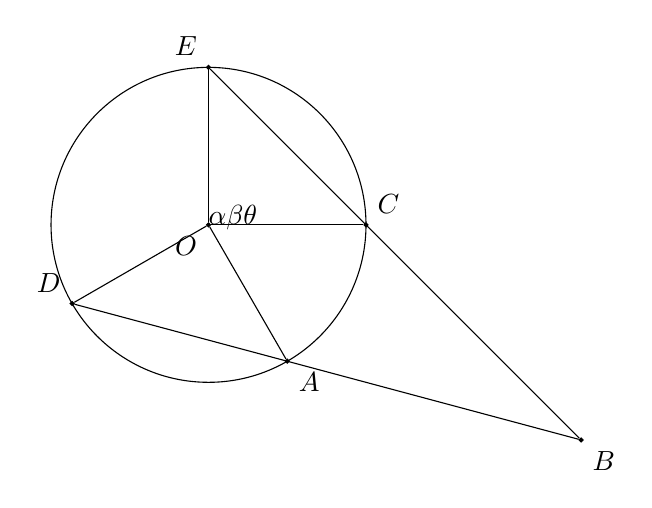
\begin{tikzpicture}
[scale=0.5,>=stealth,point/.style={draw,circle,fill = black,inner sep=0.5pt},]
%\tikzset{shift={(-3,0)}}

%innput parameters
\def\r{4}

%Labeling points
% r sin(pi/3) = 3.4641
\node (O) at (0,0)[point,label=below left:$O$] {};
\node (C) at (\r, 0 )[point,label=above right:$C$] {};
\node (A) at ({\r/2},-3.4641)[point,label=below right:$A$] {};
\node (D) at (-3.4641 , -{\r/2})[point,label=above left:$D$] {};
\node (E) at (0 , \r)[point,label=above left:$E$] {};
\node (B) at (9.4641 , -5.4641)[point,label=below right:$B$] {};


%A



%Drawing parallelogram ABCD
\draw (O) -- (A);
\draw (O) -- (C);
\draw (O) -- (E);
\draw (O) -- (D);
\draw (D) -- (B);
\draw (E) -- (B);
%\draw (C) -- (D);


\draw (O) circle (\r);
%marking angles
\tkzMarkAngle[fill=orange!50,mark=](E,O,D)
\tkzMarkAngle[fill=green!50,mark=](A,O,C)
\tkzLabelAngle[pos=0.65](E,O,D){$\alpha$}
\tkzLabelAngle[pos=0.65](A,O,C){$\beta$}
%\tkzMarkAngle[fill=orange!50,mark=](E,B,D)
\tkzLabelAngle[pos=2.65](E,B,D){$\theta$}

%
\end{tikzpicture}
}
\caption{}
\label{fig:8.5.49_circle}	
\end{figure}
%
\item {\em Construction: }See Fig. \ref{fig:8.5.49_circle}.  The input parameters are
%
\begin{align}
\label{eq:8.5.49_constr_o}
\vec{O} &= \myvec{0\\0} 
\\
\vec{C} &= \myvec{r\\0} 
\label{eq:8.5.49_constr_c}
\end{align}
Then, 
%
\begin{align}
\label{eq:8.5.49_constr_a}
\vec{A} &= r\myvec{\cos \beta \\ -\sin \beta} 
\end{align}

\subitem Equal chords subtend equal angles at the centre.  Hence 
\begin{align}
\phase{EOC} &= \phase{AOD} = \frac{360 \degree - \alpha -\beta}{2}
\\
&= 180\degree - \frac{\alpha+\beta}{2}
\end{align}
Thus, 
\begin{align}
\vec{D} &= r\myvec{\cos \brak{180^{\circ}-\frac{\alpha+\beta}{2}+\alpha} \\ \sin \brak{180^{\circ}-\frac{\alpha+\beta}{2}+\alpha}} 
\\
 &= r\myvec{-\cos \frac{\alpha-\beta}{2} \\ -\sin \frac{\alpha-\beta}{2}}
\label{eq:8.5.49_constr_d}
\\
\vec{E} &= r\myvec{\cos \brak{180^{\circ}-\frac{\alpha+\beta}{2}} \\ \sin \brak{180^{\circ}-\frac{\alpha+\beta}{2}}}
\\
 &= r\myvec{-\cos \frac{\alpha+\beta}{2} \\ \sin \frac{\alpha+\beta}{2}}
\label{eq:8.5.49_constr_e}
\end{align}
\subitem $\vec{B}$ can be found as the intersection of $AD$ and $CE$.

\item {Proof: } From 
\eqref{eq:8.5.49_constr_a},
\eqref{eq:8.5.49_constr_c},
\eqref{eq:8.5.49_constr_d} and 
\eqref{eq:8.5.49_constr_e}
\begin{align}
\vec{C}-\vec{E} &= r \myvec{1 + \cos\brak{\frac{\alpha+\beta}{2}}\\ -\sin \brak{\frac{\alpha+\beta}{2}}}
\\
&= 2r \cos\brak{\frac{\alpha+\beta}{4}} \myvec{\cos\brak{\frac{\alpha+\beta}{4}}\\ -\sin \brak{\frac{\alpha+\beta}{4}}} \quad \text{ and }
\label{eq:8.5.49_ce}
\\
\norm{\vec{C}-\vec{E}} &= 2r \cos\brak{\frac{\alpha+\beta}{4}}
\label{eq:8.5.49_cenorm}
\end{align}
and 
\begin{align}
\vec{A}-\vec{D} &= r \myvec{\cos \beta + \cos\brak{\frac{\alpha-\beta}{2}}\\ -\sin \beta+\sin \brak{\frac{\alpha-\beta}{2}}}
\\
&= 2r \cos\brak{\frac{\alpha+\beta}{4}} \myvec{ \cos \brak{\frac{\alpha-3\beta}{4}} \\ \sin \brak{\frac{\alpha-3\beta}{4}}} \text{ and }
\label{eq:8.5.49_ad}
\\
\norm{\vec{A}-\vec{D}} &= 2r \cos\brak{\frac{\alpha+\beta}{4}}
\label{eq:8.5.49_adnorm}
\end{align}
Thus, 
\begin{align}
\cos \phase{B} &= \frac{\brak{\vec{A}-\vec{D}}\brak{\vec{C}-\vec{E}}}{\norm{\vec{A}-\vec{D}}\norm{\vec{C}-\vec{E}}}
\\
&= \cos \brak{\frac{\alpha-\beta}{2}}
\\
\implies \phase{B} &= \frac{\alpha-\beta}{2}
\end{align}
%
upon substituting from \eqref{eq:8.5.49_ad},
\eqref{eq:8.5.49_adnorm},
\eqref{eq:8.5.49_ce},
\eqref{eq:8.5.49_cenorm} and simplifying.


\end{enumerate}

\item Prove that the circle drawn with any side of a rhombus as diameter, passes through
the point of intersection of its diagonals.
\item $ABCD$ is a parallelogram. The circle through $A, B$ and $C$ intersect $CD$ (produced if
necessary) at $E$. Prove that $AE = AD$.
\item $AC$ and $BD$ are chords of a circle which bisect each other. Prove that (i) $AC$ and $BD$ are
diameters, (ii) $ABCD$ is a rectangle.
\item Bisectors of angles $A, B$ and $C$ of a $\triangle ABC$ intersect its circumcircle at $D, E$ and
$F$ respectively. Prove that the angles of the $\triangle DEF$ are $90\degree – \frac{A}{2}, 90\degree – \frac{B}{2}$ and $90\degree – \frac{C}{2}$.
\item Two congruent circles intersect each other at points A and B. Through A any line segment PAQ is drawn so that $P, Q$ lie on the two circles. Prove that $BP = BQ$.
\item In any $\triangle ABC$, if the angle bisector of $\angle A$ and perpendicular bisector of $BC$ intersect, prove that they intersect on the circumcircle of the $\triangle ABC$.
%
\item The lengths of tangents drawn from an external point to a circle are equal.
%
\item Prove that in two concentric circles, the chord of the larger circle, which touches the smaller circle, is bisected at the point of contact.
%
\item Two tangents $TP$ and $TQ$ are drawn to a circle with centre $O$ from an external point $T$. Prove that $\angle PTQ = 2 \angle OPQ$.
%
\item Prove that the tangents drawn at the ends of a diameter of a circle are parallel. 
\item  Prove that the perpendicular at the point of contact to the tangent to a circle passes through the centre.
\item A quadrilateral $ABCD$ is drawn to circumscribe a circle. Prove that 
$AB + CD = AD + BC$.
%
\item $XY$ and $X'Y'$ are two parallel tangents to a circle with centre $O$ and another tangent $AB$ with point of contact $C$ intersecting $XY$ at $A$ and $X'Y'$ at $B$. Prove that $\angle AOB = 90\degree$
\item Prove that the angle between the two tangents drawn from an external point to a circle is supplementary to the angle subtended by the line-segment joining the points of contact at the centre.
\item  Prove that the parallelogram circumscribing a circle is a rhombus.
%
\item Prove that opposite sides of a quadrilateral circumscribing a circle subtend supplementary angles at the centre of the circle.
%
\item Find the area of a sector of angle $p$ (in degrees) of a circle with radius $R$. 
\item  Two chords $AB$ and $CD$ intersect each other at the point $P$. Prove that : 
\begin{enumerate}
\item   $\triangle  APC  \sim   \triangle  DPB$
\item  $AP . PB = CP . DP$
\end{enumerate}
\item Two chords $AB$ and $CD$ of a circle intersect each other at the point $P$ (when produced) outside the circle. Prove that 
\begin{enumerate}
\item   $\triangle  PAC  \sim   \triangle  PDB$
\item  $PA . PB = PC . PD$
\end{enumerate}

\end{enumerate}
